\documentclass[tikz]{standalone}

\usepackage{pgfplots}
\pgfplotsset{compat=newest}

\usepackage{tkz-tab}
\usepackage{amsmath}

\begin{document}

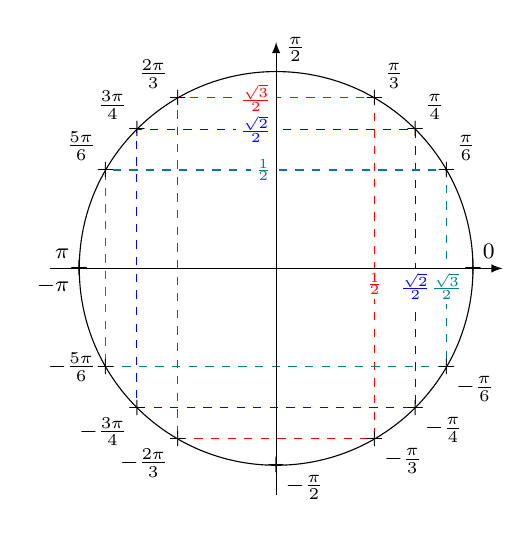
\begin{tikzpicture}[scale=2.5]
	\draw[color=red,dashed] (-1/2,-0.8660254038) -- (1/2,-0.8660254038) -- (1/2,0.8660254038) -- (-1/2,0.8660254038) -- (-1/2,-0.8660254038);
	\draw[color=blue,dashed] (-0.7071067812,-0.7071067812) -- (0.7071067812,-0.7071067812) -- (0.7071067812,0.7071067812) -- (-0.7071067812,0.7071067812) -- (-0.7071067812,-0.7071067812);
	\draw[color=teal,dashed] (-0.8660254038,-1/2) -- (0.8660254038,-1/2) -- (0.8660254038,1/2) -- (-0.8660254038,1/2) -- (-0.8660254038,-1/2);
	\draw (1,0) node {\footnotesize$+$} node[anchor=south west] {\footnotesize $0$};
	\draw (-1,0) node {\footnotesize$+$} node[anchor=south east] {\footnotesize $\pi$};
	\draw (-1,0) node {\footnotesize$+$} node[anchor=north east] {\footnotesize $-\pi$};
	\draw (0,1) node[anchor=south west] {\footnotesize $\frac{\pi}{2}$};
	\draw (1/2,0.8660254038) node {\footnotesize$+$} node[anchor=south west] {\footnotesize $\frac{\pi}{3}$};
	\draw (0.7071067812,0.7071067812) node {\footnotesize$+$} node[anchor=south west] {\footnotesize $\frac{\pi}{4}$};
	\draw (0.8660254038,1/2) node {\footnotesize$+$} node[anchor=south west] {\footnotesize $\frac{\pi}{6}$};
	\draw (-1/2,0.8660254038) node {\footnotesize$+$} node[anchor=south east] {\footnotesize $\frac{2\pi}{3}$};
	\draw (-0.7071067812,0.7071067812) node {\footnotesize$+$} node[anchor=south east] {\footnotesize $\frac{3\pi}{4}$};
	\draw (-0.8660254038,1/2) node {\footnotesize$+$} node[anchor=south east] {\footnotesize $\frac{5\pi}{6}$};
	\draw (0,-1) node {\footnotesize$+$} node[anchor=north west] {\footnotesize $-\frac{\pi}{2}$};
	\draw (1/2,-0.8660254038) node {\footnotesize$+$} node[anchor=north west] {\footnotesize $-\frac{\pi}{3}$};
	\draw (0.7071067812,-0.7071067812) node {\footnotesize$+$} node[anchor=north west] {\footnotesize $-\frac{\pi}{4}$};
	\draw (0.8660254038,-1/2) node {\footnotesize$+$} node[anchor=north west] {\footnotesize $-\frac{\pi}{6}$};
	\draw (-1/2,-0.8660254038) node {\footnotesize$+$} node[anchor=north east] {\footnotesize $-\frac{2\pi}{3}$};
	\draw (-0.7071067812,-0.7071067812) node {\footnotesize$+$} node[anchor=north east] {\footnotesize $-\frac{3\pi}{4}$};
	\draw (-0.8660254038,-1/2) node {\footnotesize$+$} node[anchor= east] {\footnotesize $-\frac{5\pi}{6}$};
	\draw (1/2,0) node[anchor=north,inner sep=1.5pt,fill=white] {\tiny \textcolor{red}{$\frac{1}{2}$}};
	\draw (0.7071067812,0) node[anchor=north,inner sep=1.5pt,fill=white] {\tiny \textcolor{blue}{$\frac{\sqrt{2}}{2}$}};
	\draw (0.8660254038,0) node[anchor=north,inner sep=1.5pt,fill=white] {\tiny \textcolor{teal}{$\frac{\sqrt{3}}{2}$}};
	\draw (0,1/2) node[anchor=east,inner sep=1.5pt,fill=white] {\tiny \textcolor{teal}{$\frac{1}{2}$}};
	\draw (0,0.7071067812) node[anchor=east,inner sep=1.5pt,fill=white] {\tiny \textcolor{blue}{$\frac{\sqrt{2}}{2}$}};
	\draw (0,0.8660254038) node[anchor=east,inner sep=1.5pt,fill=white] {\tiny \textcolor{red}{$\frac{\sqrt{3}}{2}$}};
	\filldraw[fill opacity=0,->] (0,0) circle (1);
	\draw[>=latex,->] (0,-1.15) -- (0,1.15);
	\draw[>=latex,->] (-1.15,0) -- (1.15,0);
\end{tikzpicture}

\end{document}